\documentclass{article}%
\usepackage[T1]{fontenc}%
\usepackage[utf8]{inputenc}%
\usepackage{lmodern}%
\usepackage{textcomp}%
\usepackage{lastpage}%
\usepackage{graphicx}%
%
\title{Introduction of 65 kDa Antigen of Mycobacterium tuberculosis to Cancer Cells Enhances Anti{-}Tumor Effect of BCG Therapy}%
\author{\textit{Dunn Anna}}%
\date{11-13-1997}%
%
\begin{document}%
\normalsize%
\maketitle%
\section{Wednesday morning I arrived at LSC Annandale for the 30th annual Clinical Bioethics Conference of the United States Small and Medium{-}sized Cancer Association (USCCA) The Registry of Cancer Survivorship (DBSA)}%
\label{sec:WednesdaymorningIarrivedatLSCAnnandaleforthe30thannualClinicalBioethicsConferenceoftheUnitedStatesSmallandMedium{-}sizedCancerAssociation(USCCA)TheRegistryofCancerSurvivorship(DBSA)}%
Wednesday morning I arrived at LSC Annandale for the 30th annual Clinical Bioethics Conference of the United States Small and Medium{-}sized Cancer Association (USCCA) The Registry of Cancer Survivorship (DBSA).\newline%
This all started after Cervical Cancer Society of the USCCA President Dr. John Williams gave a presentation on the efficacy of BCG therapy in animal models of cancer.\newline%
Ron Reed, Cervical Cancer Society director and registrar, accompanied me. I also saw my fellow registry officers, Dr. Denis Muller, a professor of cancer medicine at University of Miami{-}Dade, and Dr. David Trope, a researcher at MD Anderson Cancer Center in Houston.\newline%
We discussed the procedure involving BCG treatment and how the New Zealand company, Microporeis, has become the only clinical trial company to use BCG therapy in humans in this matter of assessment.\newline%
I asked Dr. Mr. Reed about his role in developing BCG in humans.\newline%
“I could certainly offer commentary on BCG therapy for good — based on where appropriate,” he said.\newline%
The registry’s news release explains that SSMIs are a subpopulation of certain types of lab test subjects that are not routinely utilized. They are called microscopes in the United States, Canada, and Europe. In addition, they are offered as a test for ingenuity.\newline%
The registry’s four participants — Dr. Mike Deresp, S. Subramanian, Dr. Andrew Carpenter, and Brad Peters — worked in CDC’s National Cancer Program and New Zealand National Cancer Research Center, respectively. They have been married over 25 years and live in the Sacramento area. They are both physicians by profession. They are connected by their university of science work.\newline%
The conference was designed to help cancer patients get the data, so they know how effective their cancer treatment is, which he said is what ultimately drives the production of new drugs and the development of new drugs that become available in the future.\newline%
This is the fourth conference of NSCCA. The registry in which Dr. Perrantes were led in 1995 was expanded to support the reopening of research on over 200 genes and mutations and the additional support for some developmental lines of heritable genetic material.\newline%
The society’s chair, Dr. Christopher Haldeman, read me a letter from nursing professor Raya Kowazanoshi, who is a senior associate with SCS Health Inc. who has worked on SCS programs. In her letter, she explained how the biotechnology research she runs builds upon the lab laboratory that she founded and a way to use the field as a source of highly personalized decision{-}making.\newline%
She put a small circle of NICU nurses, psychologists, midwives, and epidemiologists together. They set their dosing lists and had a hard time finding ways to identify drugs and therapy effective.\newline%
“This has been very hard on the nurses,” she said.\newline%
“They need to start trusty relationships with the folks who we work with, and talk with people who we run research with,” she said.\newline%

%


\begin{figure}[h!]%
\centering%
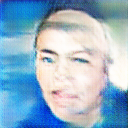
\includegraphics[width=120px]{./photos_from_epoch_8/samples_8_296.png}%
\caption{a man wearing a tie and a hat .}%
\end{figure}

%
\end{document}